\documentclass[12pt]{article}
\usepackage[utf8]{inputenc}
\usepackage[english, russian]{babel}
\usepackage{graphicx, float, multicol, hyperref, pgfplots}

\title{Определение модуля Юнга на основе исследования деформаций растяжения и изгиба}
\author{Балдин Виктор}

\begin{document}
    \maketitle

    \section{Aннотация}
    \textbf{Цель работы:} экспериментально получить зависимость между напряжением и деформацией
    для двух простейших напряженных состояний упругих тел: одностороннего сжатия и чистого изгиба;
    по результатам эксперимента вычислить модул Юнга.\\
    \textbf{В работе используются:} в первой части - прибор Лермантова, проволока
    из исследуемого материала,
     зрительная трубка со шкалой,
    набор грузов, микрометр, рулетка;  во второй части - стойка для изгибания балки, индикатор для
    измерения величин прогиба,
набор исследуемых стержней, грузы, линейка, штангенциркуль.

    \section{Определение модуля Юнга по измерениям растяжения проволоки}
    \subsection{Теоретические сведения}
    Растяжение проволоки соответствует напряженному состоянию вдоль одной оси, которое описывается формулой:
\begin{equation}
    \frac{F}{S} = E \frac{\Delta l}{l}
    \label{lermantov}
\end{equation}
Измерения производятся на установке Лермантова.
Направим зрительную трубку на зеркальце.
Тогда учитывая параксиальность углов,
для расчета растяжения проволоки справедлива формула:
\begin{equation}
    l = n\frac{r}{2h},
    \label{dlina}
\end{equation}
где $h$ - расстояние от шкалы до зеркальца,
$r$ - длина рычага, n - показания шкалы\\

    \subsection{Методика измерений}
    \begin{figure}[H]
        \centering
        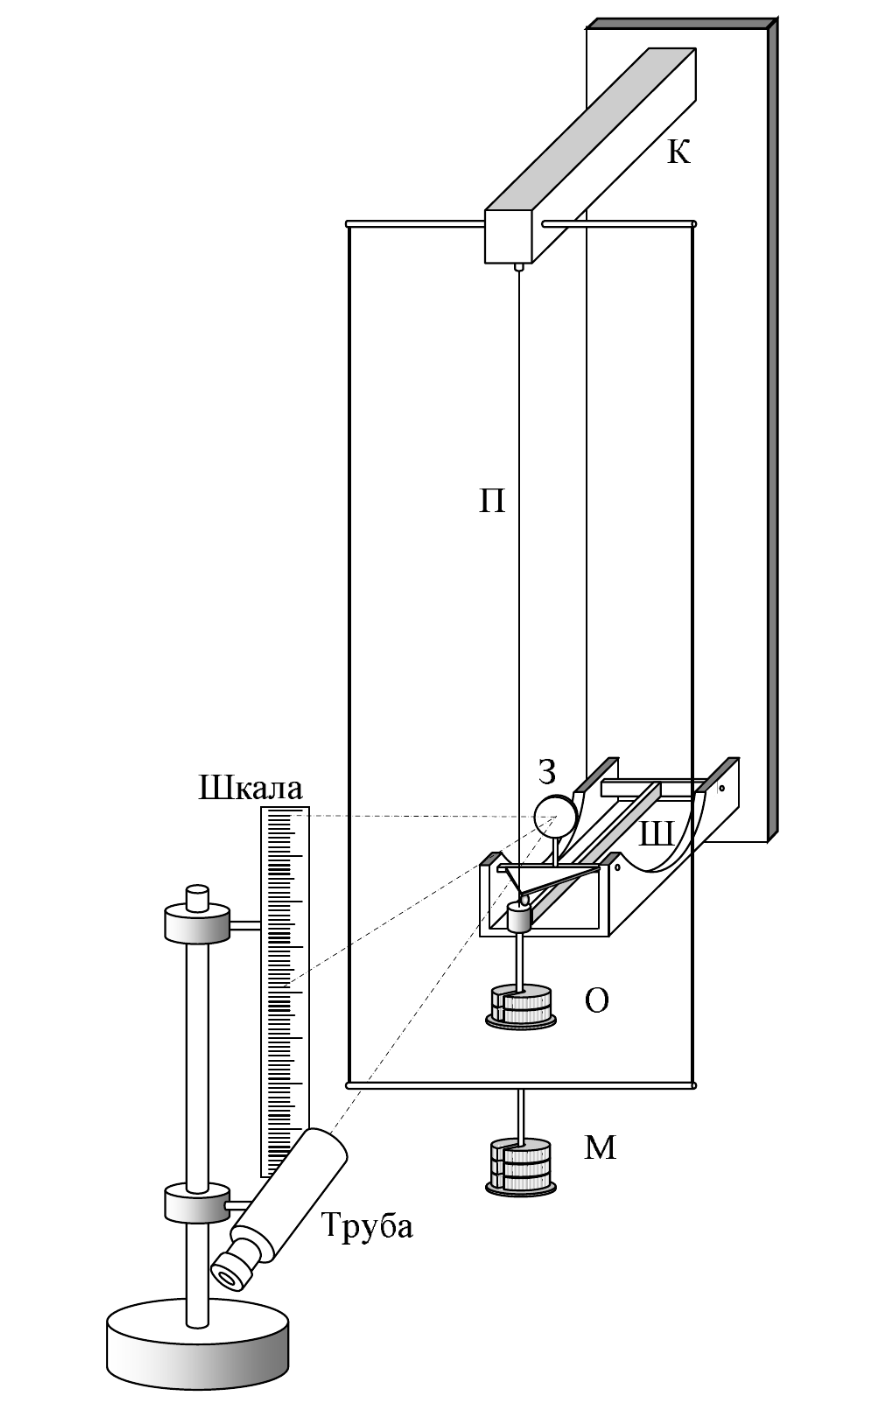
\includegraphics[scale = 0.3]{pictures/lermantov.png}
        \caption{Прибор Лермантова}
    \end{figure}

    Для определения модуля Юнга используется прибор Лермонтова,
    схема которого изображена на рис. 1. Верхний конец проволоки П, изготовленной
    из исследуемого материала, прикреплен к консоли К, а
    нижний -- к цилиндру, которым оканчивается шарнирный кронштейн
    Ш. На этот же цилиндр опирается рычаг r, связанный с зеркальцем
    3. Таким образом, удлинение проволоки можно измерить по углу
    поворота зеркальца.\\
    Натяжение проволоки можно менять, перекладывая грузы с
    площадки М на площадку О и наоборот. Такая система позволяет
    исключить влияние деформации кронштейна К на точность измерений, так
    как нагрузка на нем все время остается постоянной.

    % \subsection{Результаты измерений и обработка данных}
    \section{Определение модуля Юнга по измерениям изгиба балки}
    \subsection{Теоретические сведения}
    Модуль Юнга материала стержня $E$ связан со стрелой прогиба $y_{max}$ как:
    \begin{equation}\label{balka}
        E=\frac{Pl^3}{4ab^3y_{max}}
    \end{equation}
    где $P$ - нагрузка на стержень, $l$ - расстояние меду точками опоры,
    $a$ - ширина балки, $b$ - высота балки.

    \subsection{Экспериментальная установка}
    Экспериментальная установка состоит из прочной стойки с
    опорными призмами А и Б (рис. 2). На ребра призм опирается исследуемой
    стержень (балка) В. В середине стержня на призме Д подвешена площадка
    П с грузами. Измерять стрелу прогиба можно с помощью индикатора И, укрепляемого
    на отдельной штанге. Полный оборот большой
    стрелки индикатора соответствует 1 мм и одному делению малого циферблата.
    \par Для исключения ошибок, возникающих вследствие прогиба стола
    при изменении нагрузки на стержень, грузы перед началом эксперимента
    лучше расположить на рейке над нижней полкой опорной стойки.
    \begin{figure}[H]
        \centering
        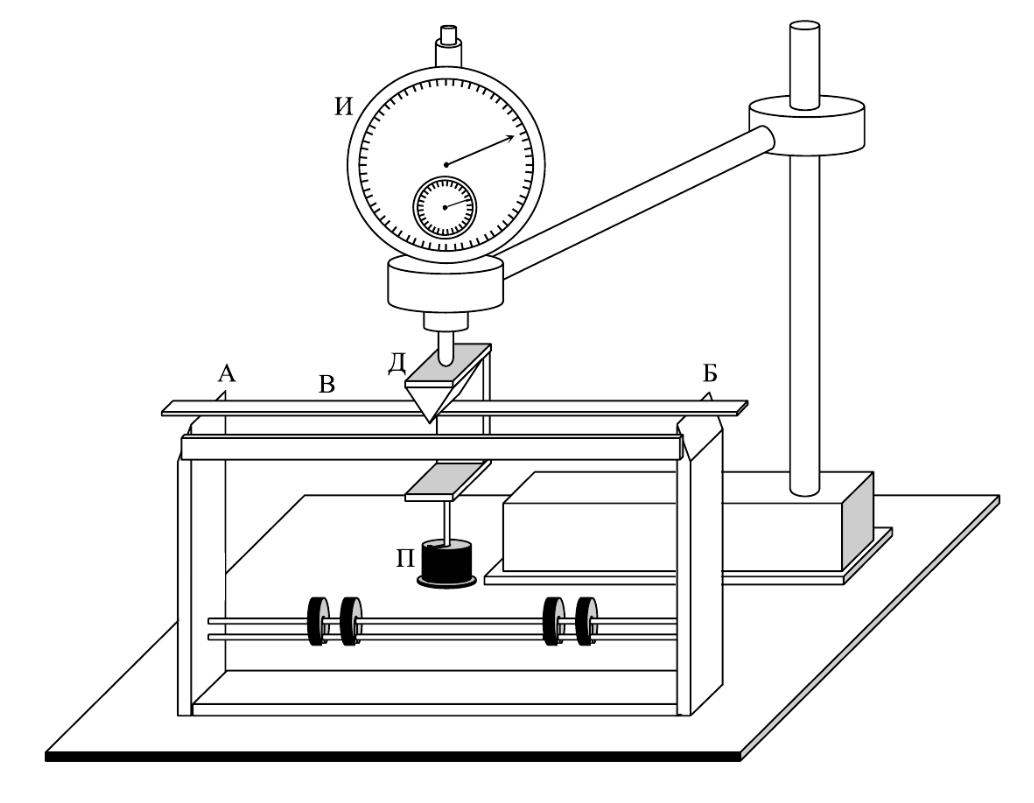
\includegraphics[scale = 0.3]{pictures/balka.png}
        \caption{Схема установки для измерения модуля Юнга}
    \end{figure}

\end{document}
